\documentclass[section, oneside]{oblivoir}
\usepackage{kotex}

% 뭐임
\usepackage{amsmath}
\usepackage{amssymb}
\usepackage{amsthm}
\usepackage{graphicx}
\usepackage{mathtools}

%--------- 멋대로 정의해본 명령어
\newcommand{\dx}[1]{\operatorname{d}\! #1}
\newcommand{\term}[1]{\textbf{#1}}


\title{푸리의 변환의 수학적 원리}
\author{esctabcapslock }

\begin{document}
\maketitle


이 상태로 보고서를 마무리하기에는, 푸리에 변환 자체를 수학적으로 접근하지 않은 것과, 내가 사용한 알고리즘에 대해 잘 모른다는 사실이 마음에 걸렸음.
따라서, 위의 탐구를 다 마친 뒤, 푸리에 변환에 관한 수학 이론적인 조사를 추가로 진행함.

※ https://blog.myungwoo.kr/54의 자료를 나름대로 이해, 본인 수준의 언어로 정리한 것임.


\section{변환이 성립하는 직관적 이유 }

\subsection{적당한 삼각함수 만들기}
푸리에 변환의 입출력 데이터를 각각 $N$차원 복소벡터공간 $\mathbb{C}^N$의 원소로 생각하자.
각 백터 $a$의 $k$번째 성분을 $a[k]$라고 표기하겠다.
그리고 두 복소 백터의 내적을 다음과 같이 정의하자
$$\left\langle a|b \right\rangle = \sum _{n=0}^{N-1} a [n] \overline{ b[n]} \quad \text{(}\bar{b}\text{는 }b\text{의 컬례 복소수)}$$
그리고 $\phi_{k}$를 다음과 같이 정의하자.
$$\phi_k \left[n \right] = \exp \left( \frac{2 \pi k}{N} n i \right) =w _{N}^{kn} \quad (w _{N}\text{은 1의 }N\text{제곱근)}$$
그려면, 임의의 정수 $k$, $l$ (단,$k \neq l$ )에 대해서,$ \left\langle \phi_k | \phi_l \right\rangle = 0$  성립.


\subsection{직교성 증명} \label{chap:ortho}

\paragraph{$k \ne l$ 일때}
$$\left\langle \phi_k | \phi_l \right\rangle = \sum_{n=0}^{N-1} \exp \left(\frac{ 2 \pi k}{N} ni \right)  \exp \left( - \frac{ 2 \pi l}{N} ni \right)$$
$$ = \sum_{n=0}^{N-1} \exp \left(\frac{ 2 \pi (k-l)}{N} ni \right) $$
$$ = \frac{ \exp ( 2\pi(k-l)i) - 1}{\exp \left( \frac{2\pi}{N} (k-l)i\right)-1} =0$$
 
\paragraph{$k=l$일때,}
$$\left\langle \phi_k \phi_k \right\rangle = \sum_{n=0}^{N-1} \exp(0) = N$$


즉, $\phi_0$, $\phi_1$, $\cdots$,  $\phi_{N-1}$은 서로 직교하니까, $\mathbb{C}^N$의 직교기저가 된다.


\subsection{이산 푸리에 변환의 정의}  \label{chap:dffuri}
푸리에 변환의 입력 데이터가 $a$, 출력 결과가 $A$라면, 푸리에 변환은 다음과 같이 표현할 수 있다.
$$A[n] = \sum_{k=0}^{N-1} a[k] {\phi_n [k]} = \left\langle a | \overline{\phi_n} \right\rangle  $$
즉, 푸리에 변환이란 기존의 백터 $a$를, 새로운 기저 $\phi_0$, $\phi_1$, $\cdots$,  $\phi_{N-1}$들을 활용해 새롭게 표현한 것이라고 이해할 수 있다.


\section{푸리에 역변환 증명}

\subsection{공식}
푸리에 변환의 역변환은 다음과 같이 구할 수 있다. 
$$a[n] = \frac{1}{N} \left\langle A[k] | \phi_k \right\rangle$$

\subsection{증명}
$$ \left\langle A | \phi_l \right\rangle = \sum _{n=0}^{N-1}  A[n] \overline{\phi_l [n] } $$

$$
=\sum_{n=0}^{N-1} \left\langle a | \overline{\phi_n} \right\rangle \overline{\phi_l [n] }   \quad ( \because \text{\ref{chap:dffuri}\sectionname 에서 정의함} )$$

$$
= \sum _{n=0}^{N-1} \sum_{k=0} ^{N-1} a[k] \phi_n [k] \overline{\phi_l[n]} $$$$
= \sum _{k=0} ^{N-1}  \sum _{n=0} ^{N-1} a[k] \phi_k [n] \overline{\phi_l [n]} 
$$

$$= \sum _{k=0} ^{N-1} a[k] \left( \sum _{n=0} ^{N-1} \phi_k [n] \overline{\phi_l [n]} \right)$$$$
= \sum _{k=0} ^{N-1} a[k] \left\langle \phi_k | \phi_l \right\rangle
 =N \vec{a} [l] \quad ( \because \text{\ref{chap:ortho}\sectionname 에서 증명함 } ) $$

즉, 내적을 이용하면 쉽게 역변환을 구할 수 있다. 


\section{고속 푸리에 변환}

\subsection{점화 관계식}
$n<\frac{N}{2}$일 때,
$$A[n] = A_{even}[n] + w _N^n A_{odd}[n] $$
$$A[n + N/2] = A_{even}[n] - w _N^n A_{odd}[n] $$

\subsection{증명}

$N$이 $2$의 거듭제골 꼴일 때 생각하자.
그리고, 푸리에 변환을 간단하게 $F$로 나타내자. $F(a)= A$이렇게.

$n<N/2$인 경우를 생각하자. 
$a _{\text{even}} [n]= a[2n]$, ${a _{odd}} (n)= a_{odd}[2n+1]$로 정의하자.

$$F(a)[n]$$
$$= \left\langle a | \overline{\phi_n} \right\rangle = \sum _{k=0}^{N-1} a[k] w _N^{kn}$$
$$= \sum _{k=0}^{N/2-1} a[2k] w _N^{2kn} + \sum _{k=0} ^{N/2-1} a[2k+1] w _N^{(2k+1)n}$$
$$= \sum _{k=0}^{N/2-1} a[2k] w _N^{2kn} + w _N^n \sum _{k=0} ^{N/2-1} a[2k+1]w _N^{2kn}$$
$$=F( a _{even} )[n]+w _N^n F( a _{odd} )[n]$$

$n \ge \frac{N}{2}$인 경우, $A _{even}$과, $A _{odd}$의 주기가 $\frac{N}{2}$니까 거의 비슷한 꼴로 적을 수 있다. ``거의 비슷한''의 이유는, $w _{N}^{n}$의 부호가 바뀌는 것을 고려해야 하기 때문이다. ($w _{N}^{N/2}$ 는 복소평면상에서 $\pi$ 회전이므로 부호가 바뀜.)


이 경우에는 다음과 같이 적힌다. (통일성을 위해 다시 $n< \frac{N}{2}$로 표현함)
$$F(a)\left[n + N/2 \right] = F( a_{even} )[n] - w_N^n F( a_{odd} )[n] $$

따라서, 기존의, 길이가 $N$이였던 것을 $\frac{N}{2}$짜리 2개로 이루어진 점화식으로 표현할 수 있다. 이것이 바로 고속 푸리에 변환(FFT)의 원리이다.

\begin{figure}[ht]
    \centering
    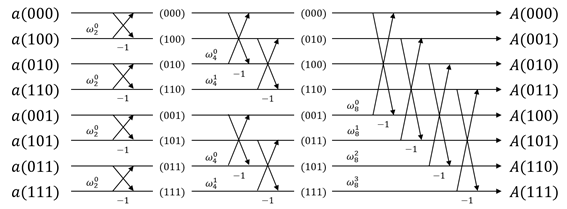
\includegraphics[width=.7\textwidth]{images/image01.png}
    \caption{콜리-튜키 알고리즘의 원리, https://casterian.net/archives/297 참조}
    \label{fig:my_label}
\end{figure}


다시 이 점화식을 컴퓨터가 계산하기 쉽도록 반복문 형태로 적절히 변형한 것이, 콜리-튜키 알고리즘, 혹은 버터플라이 알고리즘으로, 앞에서 필자가 뭣도 모르고 인터넷에서 긁어와 사용한 코드이다.



\end{document}